\documentclass{book}

% --- Packages (order matters) ---
\usepackage{titlesec}
\usepackage[table]{xcolor}
\usepackage{array}
\usepackage[colorinlistoftodos]{todonotes}
\setcounter{tocdepth}{4}
\usepackage{amsmath}
\usepackage{graphicx}
\usepackage{tikz}
\usepackage{svg}
\usetikzlibrary{graphs,graphdrawing,arrows.meta,mindmap,fit,positioning}
\usegdlibrary{layered,force}
\usepackage[edges]{forest}
\usepackage{float}
\usepackage{caption}
\captionsetup{singlelinecheck=false}
\usepackage{minted}
\usemintedstyle{friendly}
\setminted{
    fontsize=\small,
    linenos,
    breaklines,
    frame=single,
    tabsize=4,
    autogobble,
}
\setminted[python]{fontsize=\footnotesize}

% convenience
\newcommand{\filepath}[1]{\href{file://#1}{\path{#1}}}
\newcommand{\pyl}[1]{\mintinline{python}{#1}}

% --- Load hyperlink packages LAST ---
\usepackage[colorlinks=true]{hyperref}
\usepackage{bookmark}   % better control over PDF outline
\usepackage{etoolbox}   % to hook into \chapter

% reset outline root at every chapter
\pretocmd{\chapter}{\cleardoublepage\bookmarksetup{startatroot}}{}{}

% optional: control outline depth/appearance
\hypersetup{
    bookmarksopen=true,
    bookmarksopenlevel=2,
    bookmarksnumbered=true
}

% TikZ colors (unchanged)
\definecolor{mainfill}{HTML}{FFF2CC}
\definecolor{mainborder}{HTML}{D6B656}
\tikzset{
    mainnode/.style={
        draw=mainborder, fill=mainfill, rectangle, align=center,
        inner sep=5pt, rounded corners, line width=0.8pt, text=black,
    }
}

% loading pdf
\usepackage{pdfpages}


\begin{document}

%table of contents
\tableofcontents
\cite{busoniu-2008-a-comprehensive-survey-of-multi-agent-reinforcement-learning}

\section{Definition}
    Language is a system of conventional symbols (spoken, written, or signed) that enables members of a community to communicate ideas, experiences, and intentions.
    Encyclopedia Britannica
    
    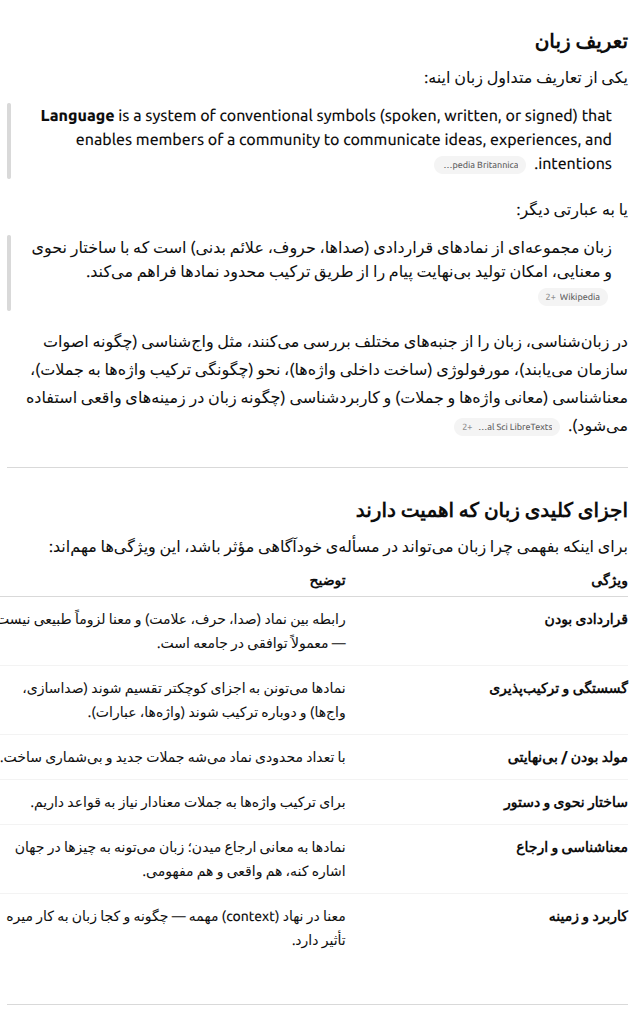
\includegraphics[width=1\linewidth]{language_definition.png}

\chapter{Biological perspective}
\url{https://www.amazon.de/-/en/dp/0199284776/?coliid=I2ZFZ3O9PPZ6RM&colid=662UPZCH1AIN&psc=1&ref_=list_c_wl_lv_ov_lig_dp_it}
    
\url{https://www.amazon.de/-/en/dp/B08B1HS3XZ/?coliid=I2QQPO9D6WJT6H&colid=662UPZCH1AIN&psc=0&ref_=list_c_wl_lv_ov_lig_dp_it}


% List todos
\listoftodos
% Bibliography
\bibliographystyle{plain}
\bibliography{refs} % Reference the BibTeX file here
\end{document}